\documentclass[12pt]{beamer}
\usetheme{LMT}
\usepackage[utf8]{inputenc}
\usepackage{amsmath}
\usepackage[makeroom]{cancel}
\usepackage{xcolor}

\setbeamertemplate{footline}[frame number]{}

\newcommand\Ccancel[2][black]{\renewcommand\CancelColor{\color{#1}}\bcancel{#2}}

\pdfinfo
{
  /Title       (Presentation Reunion)
  /Author      (Pierre NARGIL)
}

\newcommand\FontReduce{\fontsize{8}{10}\selectfont}
\newcommand\FontReduceT{\fontsize{9}{11}\selectfont}


\title{Avancement du travail}
\subtitle{Présentation hebdomadaire}
\author{Pierre Nargil}

\graphicspath{{figures/}}
% ---------------------------------------------------------------------
\begin{document}


\frame{\titlepage}

\frame{\tableofcontents}


\section{Rappels de la dernière réunion}

	\begin{frame}
	
		\frametitle{Rappels de la dernière réunion}
		%\framesubtitle{Un sous titre}
		
		\begin{itemize}
			\item Les questions abordées :
			\begin{itemize}
				\only<1>{\FontReduce}
				\item Vérifier si le premier mode en espace n'est pas toujours dédoublé par la PGD, le point fixe converge-t-il dans ces cas? 
						\\ 	\only<2>{\textcolor{blue}{le premier mode n'est pas toujours répété. 
																			Cela ne semble pas avoir de lien avec la convergence du point fixe.}}
				\item Comment est résolue la partie non linéaire du programme. Point fixe?
						\\ 	\only<3>{\textcolor{blue}{Point fixe, et cela semble poser des problèmes de convergence 
																								qui n'apparaissaient pas précédemment.}}
				\item D'où vient la différence d'ordre de grandeur entre les modes en espace sur les graphiques présentés?
						\\ 	\only<4>{\textcolor{blue}{Les modes affichés pour la POD étaient la sortie de la SVD, et temps comme espace 
																			étaient séparément multipliés par les valeurs propres associées (seulement pour l'affichage)}}
				\item \textcolor<-1>{red}{Pourquoi le nouveau mode trouvé après l'orthogonalisation est incohérent ?}
			\end{itemize}
			
			\only<-1>{
				\item Les objectifs de travail à court terme :
				\begin{itemize}
					\FontReduce
					\item Faire une SVD des modes PGD, comparer avec les modes POD.
					\item Comparer avec la solution exacte de François
					\item Résultat pour le problème de cas test linéaire 
					\item \textcolor<-1>{red}{Résultats pour les problèmes de cas test non-linéaires (POD)}
					\item \textcolor<-1>{red}{Mettre en place une résolution Newton-Raphson pour l'élément non-linéaire.}
				\end{itemize}
			}
		\end{itemize}

	\end{frame}

%\section{Point de travail - avancement}

%\section{Questions soulevées}
\section{Constats et Remarques}
	\begin{frame}
	\FontReduceT
		\frametitle{Constats et Remarques}
		\begin{itemize}
			\item Grands pas de temps \& amortissement du schéma 
				\begin{itemize}
					\FontReduce
					\item négatif pour la convergence de la PGD vers la solution complète et ralentissent
					\item ralenti également le point fixe
				\end{itemize}
			
			\item Les fonctions d'effet de butée
				\begin{itemize}
					\FontReduce
					\item $\frac{k}{\alpha} \left( e^{\alpha (u-j)} - 1 \right) \Ccancel[red]{ + k j} + k u $
					\item 	$F(u) = k u \text{  si  } u < j $ \\
							 	$ \phantom{F(u)} = \frac{k \Delta j^2}{(u-j)-\Delta j} + k (j - \Delta j)	\text{  sinon}$
					\item Définition par morceau / Définir $\mathbf{K}$ / Valeur au delà de la limite.
					\item raideur proposée : $k \alpha \left( e^{\alpha (u-j)} - 1 \right) + k $
				\end{itemize}
			\item Présence sur la partie non-linéaire d'oscillations haute fréquence au début du calcul
			\item Une fois en butée l'élément ne semble pas pouvoir retourner en arrière (trop grande rigidité? Orienter la résistance à l'effort ?)
		\end{itemize}
	\end{frame}
%\section{Idées}
%	\begin{frame}
%		\frametitle{Idées}
%		\begin{itemize}
%			\item $\circ$ Supprimer les modes PGD non convergés ?
%		\end{itemize}
%	\end{frame}
\section{Modifications dans le programme}
	\begin{frame}
		\frametitle{Modifications dans le programme}
		\begin{itemize}
			\item $\bullet$ Afficher les modes de POD redressés plutôt que la sortie de SVD
			\item $\bullet$ Prendre en compte les modes PGD hors point fixe dans l'affichage
			\item $\bullet$ Ajouter Ttot dans les variables de départ pour résoudre des problèmes plus "lent"
			\item $\bullet$ Utilisation d'une fonction associée à chaque non-linéarité
			\item $\circ$ Utilisation de plusieurs non-linéarités
				\begin{itemize}
					\FontReduce
					\item Stagnation du point fixe (entre deux valeurs)
					\item Augmentation de la tolérance pour passer la stagnation $\Rightarrow$ Divergence
					%\item Augmenter la "souplesse" de la butée diminue la vitesse de divergence
					\item Augmenter l'espace avant la butée semble entrainer la divergence
					\item Le problème peut se présenter aussi avec une seule non-linéarité
				\end{itemize}
		\end{itemize}
	\end{frame}
%\subsection{Presudo-programme}
%\subsection{Cas test}
%\subsection{Equations}
\section{0bjectifs de travail}

	\begin{frame}
	
		\frametitle{0bjectifs de travail}
			\framesubtitle{Comparer les modes POD à une SVD des modes PGD}
				\begin{figure}
			\only<1>{
				\includegraphics[width=0.5\linewidth ,keepaspectratio]{Beam-tikz-0.pdf}				
				\includegraphics[width=0.5\linewidth ,keepaspectratio]{SinVerse-tikz.pdf}	
				\\
				Valeur singulières
					\includegraphics[width=0.32\linewidth ,keepaspectratio]{matValeursSinguliere3.eps}
					\includegraphics[width=0.32\linewidth ,keepaspectratio]{matValeursSinguliere4.eps}
					\includegraphics[width=0.32\linewidth ,keepaspectratio]{matValeursSinguliere5.eps}
				\\
				}
			\only<2>{
				Schéma Accélération moyenne
					%\raisebox{-0.5\height}{	}
						\includegraphics[trim=1cm 0cm 0cm 0cm, clip=true,width=0.55\linewidth ,keepaspectratio]{MAC-3-PGDR-POD.pdf}
						\includegraphics[trim=0.5cm 0cm 0cm 0cm, clip=true,width=0.55\linewidth ,keepaspectratio]{MAC-3-PGDR-POD-2.pdf}
				}
			\only<3>{
				Schéma Accélération moyenne modifiée (amorti)
					\includegraphics[trim=1cm 0cm 0cm 0cm, clip=true,width=0.55\linewidth ,keepaspectratio]{MAC-4-PGDR-POD.pdf}
					\includegraphics[trim=0.5cm 0cm 0cm 0cm, clip=true,width=0.55\linewidth ,keepaspectratio]{MAC-4-PGDR-POD-2.pdf}
			}
			\only<4>{
				Schéma HHT
					\includegraphics[trim=1cm 0cm 0cm 0cm, clip=true,width=0.55\linewidth ,keepaspectratio]{MAC-5-PGDR-POD.pdf}
					\includegraphics[trim=0.5cm 0cm 0cm 0cm, clip=true,width=0.55\linewidth ,keepaspectratio]{MAC-5-PGDR-POD-2.pdf}
			}
			\only<5>{
				\begin{itemize}
					\item Modes corrélés mais non identiques
					\item La famille de modes qui subit la SVD n'est pas "hiérarchisée"
							\begin{itemize}
								\item Utiliser une famille pondérée par les normes des fonctions de temps associées ?
							\end{itemize}
				\end{itemize}
			}
				\end{figure}
	\end{frame}
	
	\begin{frame}
	
		\frametitle{0bjectifs de travail}
			\framesubtitle{Comparer les modes POD à une SVD des modes PGD (Pondérés)}
				\begin{figure}
			\only<1>{
				Problème étudié : Une poutre soumise à un sinusverse lent.
				\\
				%\vspace{1.5cm}
					\includegraphics[width=0.32\linewidth ,keepaspectratio]{NormeFonctionsTemps.eps}
					\\
					Normes des fonctions du temps
					\includegraphics[width=0.32\linewidth ,keepaspectratio]{matValeursSinguliereP3.eps}
					\includegraphics[width=0.32\linewidth ,keepaspectratio]{matValeursSinguliereP4.eps}
					\includegraphics[width=0.32\linewidth ,keepaspectratio]{matValeursSinguliereP5.eps}
				\\
				Valeur singulières
				}
			\only<2>{
				Schéma Accélération moyenne
					%\raisebox{-0.5\height}{	}
						\includegraphics[trim=1cm 0cm 0cm 0cm, clip=true,width=0.55\linewidth ,keepaspectratio]{MAC-3-PGDPR-POD.pdf}
						\includegraphics[trim=0.5cm 0cm 0cm 0cm, clip=true,width=0.55\linewidth ,keepaspectratio]{MAC-3-PGDPR-POD-2.pdf}
				}
			\only<3>{
				Schéma Accélération moyenne modifiée (amorti)
					\includegraphics[trim=1cm 0cm 0cm 0cm, clip=true,width=0.55\linewidth ,keepaspectratio]{MAC-4-PGDPR-POD.pdf}
					\includegraphics[trim=0.5cm 0cm 0cm 0cm, clip=true,width=0.55\linewidth ,keepaspectratio]{MAC-4-PGDPR-POD-2.pdf}
			}
			\only<4>{
				Schéma HHT
					\includegraphics[trim=1cm 0cm 0cm 0cm, clip=true,width=0.55\linewidth ,keepaspectratio]{MAC-5-PGDPR-POD.pdf}
					\includegraphics[trim=0.5cm 0cm 0cm 0cm, clip=true,width=0.55\linewidth ,keepaspectratio]{MAC-5-PGDPR-POD-2.pdf}
			}
			\only<5>{
				\begin{itemize}
					\item Modes corrélés très proches pour les premiers
					\item Famille plus pertinente 
				\end{itemize}
			}
				\end{figure}
	\end{frame}
	
	\begin{frame}
		\frametitle{0bjectifs de travail}
			\framesubtitle{Comparer avec la solution exacte de François}
			\only<1>{
				Présentation de François - Solution exacte
					\includegraphics[width=1\linewidth ,keepaspectratio]{ExempleLouf.png}
					\\
					\includegraphics[width=1\linewidth ,keepaspectratio]{ResultLouf.png}
			}
			\only<2>{
				Résultat de mon programme - avec les valeurs partagées
				\begin{figure}
					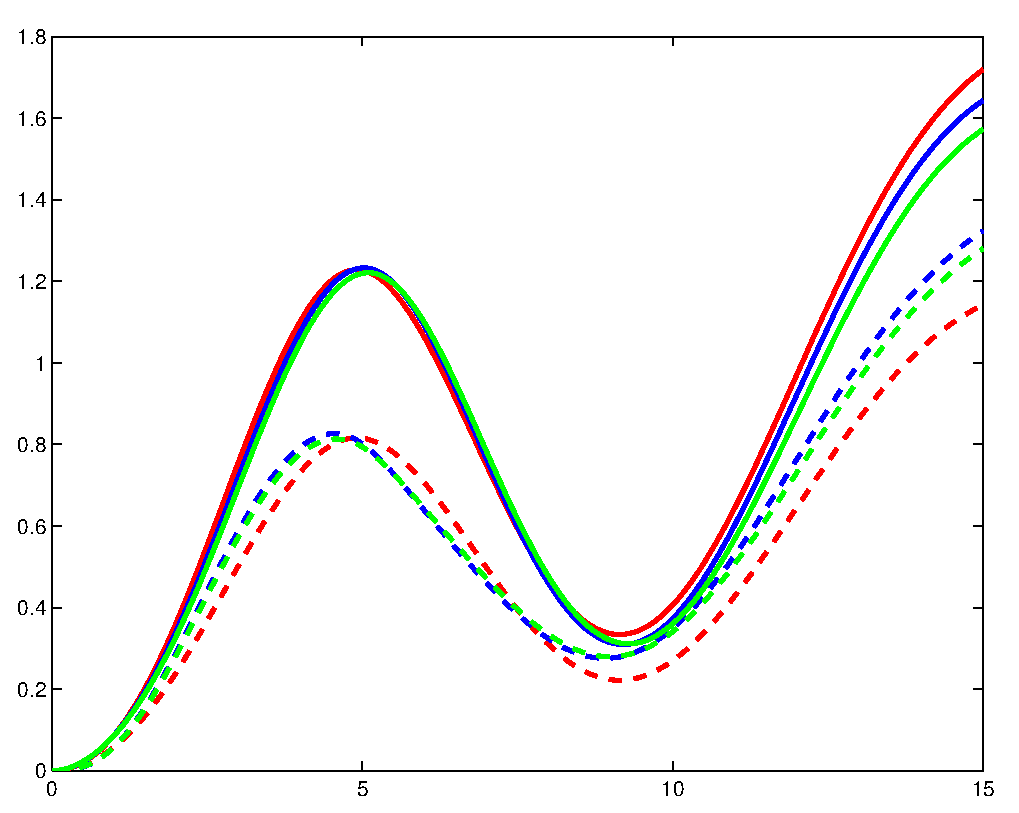
\includegraphics[width=0.75\linewidth ,keepaspectratio]{matReponseRessort.eps}				
				\end{figure}
			}
	\end{frame}
	
	\begin{frame}
		\frametitle{0bjectifs de travail}
			\framesubtitle{Résultat pour le problème de cas test 1 - linéaire }
				Le cas test, chargement sinusoïdal.
					\includegraphics[width=1\linewidth ,keepaspectratio]{CasTest1.png}
					\\
					Sur imprimés :
					\begin{itemize}
						\item POD inchangée par le schéma, solution complète trouvée avec 2 modes
						\item PGD : stagnation à $10^{-2.5}$ d'erreur, sauf pour le schéma 3
					\end{itemize}
	\end{frame}
	
	\begin{frame}
		\frametitle{0bjectifs de travail}
			\framesubtitle{Résultat pour le problème poutre - linéaire }
			\includegraphics[width=0.5\linewidth ,keepaspectratio]{Beam-tikz-0.pdf}				
			\includegraphics[width=0.5\linewidth ,keepaspectratio]{SinVerse-tikz.pdf}	
			\\
			Sur imprimés:
				\begin{itemize}
					\item Le premier mode n'est pas toujours répété. Cela ne semble pas avoir de lien avec la convergence du point fixe.
					\item Le schéma 3 semble ici aussi apporter la possibilité de réduire l'erreur sans stagnation infranchissable.
								Mais le calcul s'arrête à 80 modes
					\item Le schéma 6 (TDG) trouvant toujours le même mode semble osciller entre deux sortie du point fixe.
				\end{itemize}
	\end{frame}
	
	
\section{Points blocants}

	\begin{frame}
	
		\frametitle{Points blocants}
		
		\begin{itemize}
			\item PGD - TDG
			\item Orthogonalisation
			\item PGD \& Non-linéaire
				\begin{itemize} 
					\item Comment prendre en compte l'évolution de $ \mathbf{K} $ dans le problème en espace.
				\end{itemize}
			\item Absence d'éléments de comparaison pour les résultats non-linéaire.
		\end{itemize}
	
	\end{frame}

\section{Questions}

	\begin{frame}
	
		\frametitle{Questions}
		
		\begin{itemize}
			\item Pseudo-programme. Une norme ou un logiciel conseillé?
			\item Comment utiliser des modes trouvés en dehors de la PGD? Faire tourner le point fixe sans modifier le mode espace ?
		\end{itemize}
	
	\end{frame}
	
\section{Programme de travail}

	\begin{frame}
	
		\frametitle{Programme de travail}
		
		\begin{itemize}
			\item Newton-R...
			\item Lundi Journée Farman
			\item SVD(SoluPGD), comparer avec SVD(ModePGDPondérés). Et une orthogonalisation à la place de la SVd ?
			\item Résoudre le problème de François avec la partie poutre du programme
			\item Jouer sur $\alpha$ pour la convergence.
			\item Amortir plus, les Masses-Ressorts, et les poutres
			\item Lecture : HOSVD
			\item Voir si le 1er mode trouver par la 1ere itération du point fixe est le mode correspondant à la réponse statique de l'effort moyen.
		\end{itemize}
	
	\end{frame}
%
%
%\begin{frame}
%
%	\frametitle{Prerequisites \& Goals}
%	\framesubtitle{Knowledge is a brick wall that you raise line by line forever}
%	
%	\begin{block}{LaTeX}
%		\begin{itemize}
%			\item Obviously some basic LaTeX knowledge is necessary
%			\item Some more features will be provided here
%		\end{itemize}
%	\end{block}
%	
%	\begin{block}{Beamer}
%		\begin{itemize}
%			\item You'll learn them by looking at this presentation source
%		\end{itemize}
%	\end{block}
%	
%	\begin{block}{Goal}
%		\begin{itemize}
%			\item Learn how to make well structured slides
%			\item Using a beautiful theme
%			\item Take over the world
%		\end{itemize}
%	\end{block}
%
%\end{frame}

\end{document}
% ---------------------------------------------------------------------
